\documentclass[border=3pt]{standalone}
% Preâmbulo compartilhado pelos diagramas TikZ da aula 7 (Filtros Não Paramétricos)
\usepackage[T1]{fontenc}
\usepackage[utf8]{inputenc}
\usepackage{lmodern}
\usepackage{amsmath}
\usepackage{xcolor}
\usepackage{tikz}
\usetikzlibrary{arrows.meta,angles,quotes,decorations.pathmorphing,calc,
                positioning,shapes.geometric,shapes.misc,backgrounds,fit,
                math}

% Paleta (mesma dos SVGs originais)
\definecolor{dblue}{HTML}{2A5B8C}
\definecolor{dorange}{HTML}{B3541E}
\definecolor{dgreen}{HTML}{4A7C59}
\definecolor{dred}{HTML}{9C4B4B}
\definecolor{dcream}{HTML}{F4F1EA}
\definecolor{dshade}{HTML}{DDD7C9}

% Função gaussiana (não normalizada por padrão de escala visual)
\pgfmathdeclarefunction{gauss}{3}{%
  \pgfmathparse{1/(#3*sqrt(2*pi))*exp(-((#1-#2)^2)/(2*#3^2))}%
}

% Estilos comuns (prefixo d... para não colidir com chaves internas do pgf)
\tikzset{
  >={Stealth[length=2mm]},
  dguide/.style={gray!55, dashed, line width=0.4pt},
  daxis/.style={gray!60, line width=0.7pt, ->},
  dbody/.style={fill=black!3, draw=black!80, line width=1pt},
  dacc/.style={draw=dblue, line width=1pt},
  dlbl/.style={black!55, font=\small},
  dsub/.style={black!45, font=\footnotesize},
  dstate/.style={circle, draw=black!80, fill=dcream, line width=1pt,
                 minimum size=17mm, font=\large, inner sep=1pt},
  dobs/.style={circle, draw=black!80, fill=dshade, line width=1pt,
               minimum size=14mm, font=\large, inner sep=1pt},
  dbox/.style={rounded corners=2pt, draw=black!80, fill=dcream, line width=1pt,
               align=center, inner sep=6pt},
  dop/.style={circle, draw=black!80, fill=white, line width=1pt,
              minimum size=6mm, inner sep=0pt, font=\small},
  dtrans/.style={->, dblue, line width=1pt},
  dmeas/.style={->, dorange, line width=1pt},
  dcurve/.style={line width=1pt, dblue},
  dcurveb/.style={line width=1.4pt, dorange},
}

\begin{document}
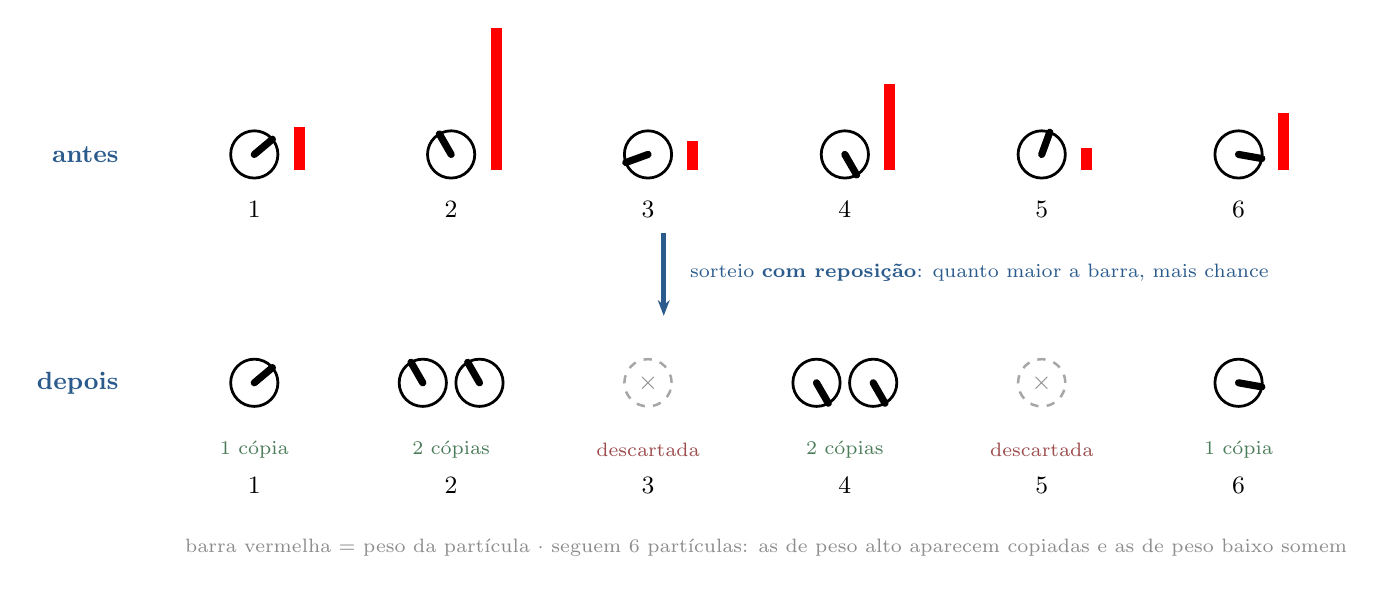
\begin{tikzpicture}[x=1cm,y=1cm]
\node[font=\small\bfseries, dblue, anchor=east] at (-0.6,3.4) {antes};\node[font=\small\bfseries, dblue, anchor=east] at (-0.6,0.5) {depois};
\begin{scope}[shift={(1.00,3.40)}]\draw[black, fill=white, line width=1pt] (0,0) circle (0.30); \draw[black, line width=2.6pt, line cap=round] (0,0) -- (40:0.30); \end{scope}
\fill[red] (1.50,3.2) rectangle ++(0.14,0.55);
\node[font=\small] at (1.00,2.7) {1};
\begin{scope}[shift={(1.00,0.50)}]\draw[black, fill=white, line width=1pt] (0,0) circle (0.30); \draw[black, line width=2.6pt, line cap=round] (0,0) -- (40:0.30); \end{scope}
\node[dgreen, font=\scriptsize] at (1.00,-0.35) {1 cópia};
\node[font=\small] at (1.00,-0.8) {1};
\begin{scope}[shift={(3.50,3.40)}]\draw[black, fill=white, line width=1pt] (0,0) circle (0.30); \draw[black, line width=2.6pt, line cap=round] (0,0) -- (120:0.30); \end{scope}
\fill[red] (4.00,3.2) rectangle ++(0.14,1.81);
\node[font=\small] at (3.50,2.7) {2};
\begin{scope}[shift={(3.14,0.50)}]\draw[black, fill=white, line width=1pt] (0,0) circle (0.30); \draw[black, line width=2.6pt, line cap=round] (0,0) -- (120:0.30); \end{scope}
\begin{scope}[shift={(3.86,0.50)}]\draw[black, fill=white, line width=1pt] (0,0) circle (0.30); \draw[black, line width=2.6pt, line cap=round] (0,0) -- (120:0.30); \end{scope}
\node[dgreen, font=\scriptsize] at (3.50,-0.35) {2 cópias};
\node[font=\small] at (3.50,-0.8) {2};
\begin{scope}[shift={(6.00,3.40)}]\draw[black, fill=white, line width=1pt] (0,0) circle (0.30); \draw[black, line width=2.6pt, line cap=round] (0,0) -- (200:0.30); \end{scope}
\fill[red] (6.50,3.2) rectangle ++(0.14,0.37);
\node[font=\small] at (6.00,2.7) {3};
\draw[black!35, dashed, line width=0.9pt] (6.00,0.5) circle (0.3); \node[black!45, font=\small] at (6.00,0.5) {$\times$};
\node[dred, font=\scriptsize] at (6.00,-0.35) {descartada};
\node[font=\small] at (6.00,-0.8) {3};
\begin{scope}[shift={(8.50,3.40)}]\draw[black, fill=white, line width=1pt] (0,0) circle (0.30); \draw[black, line width=2.6pt, line cap=round] (0,0) -- (300:0.30); \end{scope}
\fill[red] (9.00,3.2) rectangle ++(0.14,1.09);
\node[font=\small] at (8.50,2.7) {4};
\begin{scope}[shift={(8.14,0.50)}]\draw[black, fill=white, line width=1pt] (0,0) circle (0.30); \draw[black, line width=2.6pt, line cap=round] (0,0) -- (300:0.30); \end{scope}
\begin{scope}[shift={(8.86,0.50)}]\draw[black, fill=white, line width=1pt] (0,0) circle (0.30); \draw[black, line width=2.6pt, line cap=round] (0,0) -- (300:0.30); \end{scope}
\node[dgreen, font=\scriptsize] at (8.50,-0.35) {2 cópias};
\node[font=\small] at (8.50,-0.8) {4};
\begin{scope}[shift={(11.00,3.40)}]\draw[black, fill=white, line width=1pt] (0,0) circle (0.30); \draw[black, line width=2.6pt, line cap=round] (0,0) -- (70:0.30); \end{scope}
\fill[red] (11.50,3.2) rectangle ++(0.14,0.28);
\node[font=\small] at (11.00,2.7) {5};
\draw[black!35, dashed, line width=0.9pt] (11.00,0.5) circle (0.3); \node[black!45, font=\small] at (11.00,0.5) {$\times$};
\node[dred, font=\scriptsize] at (11.00,-0.35) {descartada};
\node[font=\small] at (11.00,-0.8) {5};
\begin{scope}[shift={(13.50,3.40)}]\draw[black, fill=white, line width=1pt] (0,0) circle (0.30); \draw[black, line width=2.6pt, line cap=round] (0,0) -- (350:0.30); \end{scope}
\fill[red] (14.00,3.2) rectangle ++(0.14,0.73);
\node[font=\small] at (13.50,2.7) {6};
\begin{scope}[shift={(13.50,0.50)}]\draw[black, fill=white, line width=1pt] (0,0) circle (0.30); \draw[black, line width=2.6pt, line cap=round] (0,0) -- (350:0.30); \end{scope}
\node[dgreen, font=\scriptsize] at (13.50,-0.35) {1 cópia};
\node[font=\small] at (13.50,-0.8) {6};
\draw[dtrans, line width=1.8pt] (6.2,2.4) -- (6.2,1.35); \node[dtrans, font=\scriptsize, anchor=west] at (6.4,1.9) {sorteio \textbf{com reposição}: quanto maior a barra, mais chance};
\node[dsub, font=\scriptsize] at (7.5,-1.6) {barra vermelha = peso da partícula $\cdot$ seguem 6 partículas: as de peso alto aparecem copiadas e as de peso baixo somem};
\end{tikzpicture}
\end{document}
